\chapter{Architektura i technologie}

Niniejszy rozdział został poświęcony ogólnemu opisowi architektury systemu oraz zastosowanych technologii. Dla poszczególnych wyborów zostały przedstawione przesłanki, którymi kierował się autor tej pracy. 

Istotnym czynnikiem mającym wpływ na wybór technologii oraz wzorców architektonicznych była chęć poszerzenia wiedzy autora niniejszej pracy w ich zakresie. Cechą wspólną wszystkich zastosowanych rozwiązań jest szeroki dostęp do materiałów w postaci dokumentacji oraz pozycji książkowych. 

\section{Architektura systemu}

Ze względu na potrzebę szerokiej dostępności platformy została ona zrealizowana jako system webowy w architekturze klient - serwer. Interfejsem użytkownika końcowego jest aplikacja kliencka typu SPA (ang. \textit{Single Page Application}) uruchamiana w przeglądarce internetowej. Aplikacja ta komunikuje się z API (ang. \textit{Application Programming Interface}) aplikacji serwerowej za pomocą zapytań protokołu HTTP (ang. \textit{Hypertext Transfer Protocol}).  Aplikacja serwerowa z kolei komunikuje się z bazą danych w celu odczytu oraz zapisu informacji za pomocą interfejsu JDBC (ang. \textit{Java DataBase Connectivity}). 

\begin{figure}[ht]
\centering
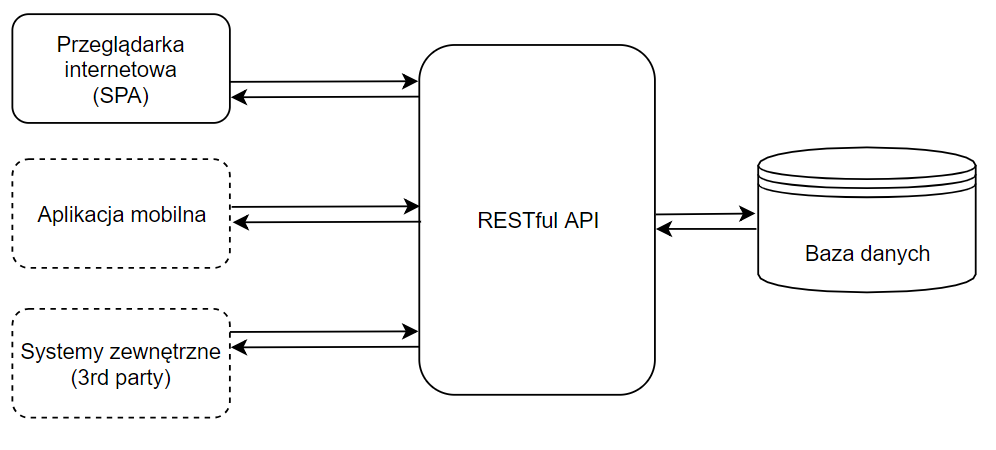
\includegraphics[width=0.8\linewidth]{05-architektura-i-technologie/rys/ogolna-architektura.PNG}
\caption{Diagram ogólnej architektury systemu}
\label{fig:diagram-og-architekt}
\end{figure}

Elementy otoczone linią kreskowaną na diagramie nie są przedmiotem tej pracy, jednak podkreślają uniwersalność API oraz wskazują możliwości rozwojowe oraz integracyjne systemu.

\subsection{RESTful API}
API wystawiane przez część serwerową zostało zaprojektowane w oparciu styl architektoniczny REST (ang. \textit{Representational State Transfer}), który zakłada komunikację klient-serwer z uwzględnieniem następujących zasad: 
\begin{itemize}
\item użycie podstawowych metody protokołu HTTP czyli - GET, PUT, POST oraz DELETE,
\item identyfikacja zasobów poprzez URL (ang. \textit{Uniform Resource Locator}),
\item komunikacja bezstanowa (brak sesji).
\end{itemize}

Użycie podstawowych metod protokołu HTTP pozytywnie wpływa na czytelność oraz intuicyjność API. Projektowanie z uwzględnieniem powyższych zasad pozwala również zminimalizować powiązania pomiędzy serwerem oraz klientem, API staje się uniwersalne. Otwiera to możliwości rozwoju systemu na inne platformy, np. utworzenie aplikacji klienckich dla systemów mobilnych Android oraz iOs. Możliwości rozwoju systemu zostały przedstawione za pomocą zakreskowanych bloków na rysunku~\ref{fig:diagram-og-architekt}

\section{Stos technologiczny}

Bla bla

\subsection{Spring Boot}

Aplikacja backendowa została zaimplementowana w języku Java (w wersji 1.8) z użyciem frameworka Spring Boot (w wersji 2.0.3). Technologie te zostały wybrane ze względu na następujące czynniki:
 \begin{itemize}
\item rozwiązania open source,
\item duże grono użytkowników oraz baza materiałów w sieci,
\item dobra dokumentacja,
\item duża ilość dostępnych modułów Springa np. do komunikacji z bazami danych,
\item chęć poszerzenia wiedzy na temat tych technologii.
\end{itemize}

\subsection{Swagger}

Swagger został wykorzystany do dostarczenia dokumentacji RESTowego API bla bla.

\subsection{JWT}

Technologia Json Web Token została wybrana jako sposób realizacji autoryzacji zapytań do API systemu. JWT jest technologią autoryzacji bezstanowej, przez co bardzo często jest używane do zabezpieczania końcówek REST'owych.

\subsection{MySQL} 

Relacyjna baza danych została wybrana ze względu na przewidywaną dużą ilość powiązań między encjami w systemie. MySQL od firmy Oracle jest darmowym, bezpiecznym oraz wydajnym systemem zarządzania bazą danych.  Istotnym uzasadnieniem wyboru tej technologii jest również bardzo dobra integracja z frameworkiem Spring.

\subsection{Angular}

Główną technologią wykorzystywaną po stronie front endu będzie framework do tworzenia SPA rozwijany przez Google - Angular (w wersji 6.1.0). Framework ten ułatwia budowę skalowalnych i szybkich aplikacji z bogatym interfejsem użytkownika. 

W celu usprawnienia procesu rozwoju aplikacji zostanie wykorzystana biblioteka ngrx (w wersji 6.1.0), wspomagająca zarządzanie stanem aplikacji. Wykorzystanie tej biblioteki znacznie ułatwia analizę działania aplikacji oraz diagnozowanie błędów.

A jakby tak opisac czemu nie react? Ze angular bardzo dobrze sprwadza sie przy duzej ilosci formularzy, react bardziej rendering framework?

\subsection{AntDesign - NgZorro}

\subsection{Heroku}
